\documentclass[12pt]{beamer}
\usetheme{Madrid}
\usepackage[utf8]{inputenc}
\usepackage[english]{babel}
\usepackage{amsmath}
\usepackage{amsfonts}
\usepackage{amssymb}
\usepackage{graphicx}
\usepackage[notransparent]{svg}
\usepackage{pdfpages}
\author{TRAN-THUONG Tien-Thinh}
\title{Cryptographie}
%\setbeamercovered{transparent} 
%\setbeamertemplate{navigation symbols}{} 
%\logo{} 
\institute{Lycée Hoche MP*} 
\usepackage{datetime}
\newdate{date}{05}{01}{2022}
\date{\displaydate{date}}
%\subject{} 
\begin{document}

\begin{frame}
\titlepage
\end{frame}

\begin{frame}{Plan}
    \tableofcontents
\end{frame}

\section{RSA}
\begin{frame}{RSA - présentation}
\begin{block}{}
Le chiffrement RSA est un algorithme de cryptographie asymétrique inventé en 1978. Il est nommé par les initiales de ses trois inventeurs:
\begin{enumerate}
	\item[•] Ronald RIVEST
	\item[•] Adi SHAMIR
	\item[•] Leonard ADLEMAN
\end{enumerate}
\end{block}
\begin{center}
  \includegraphics[width=200px]{RSA}
\end{center}
\end{frame}

\subsection{Fonctionnement}
\begin{frame}{RSA - clé asymétrique}
\begin{center}
  \makebox[\textwidth]{\includegraphics[width=\paperwidth]{cle asymetrique.pdf}}
\end{center}
\end{frame}

\begin{frame}{RSA - générer les clés}
\begin{center}
  \makebox[\textwidth]{\includegraphics[height=220px]{generePQ.pdf}}
\end{center}
\end{frame}

\begin{frame}{RSA - chiffrer un message}
\begin{center}
  \makebox[\textwidth]{\includegraphics[height=220px]{chiffrer.pdf}}
\end{center}
\end{frame}

\begin{frame}{RSA - déchiffrer un message}
\begin{center}
  \makebox[\textwidth]{\includegraphics[height=220px]{dechiffrer.pdf}}
\end{center}
\end{frame}

\begin{frame}{RSA - démonstration}
	Montrer que $M^{d\times e} \equiv M [p \times q]$ \\ Revient à démontrer que $M^{d\times e} \equiv M [p]$ et $M^{d\times e} \equiv M [q]$
	\begin{alertblock}{Petit Théorème de Fermat}
p premier, alors, $\forall a \in N$ non divisible par p, $a^{p-1} \equiv 1 [p]$

	\end{alertblock}
	\begin{block}{Si $M \equiv 0 [p]$}
	$M^{d\times e} \equiv 0 \equiv M [p]$
	\end{block}
	\begin{block}{Si $M \not\equiv 0 [p]$}
On sait que $e\times d \equiv 1 [\varphi(n)]$ or $\varphi(n)=(p-1)(q-1)$ d'où $\exists k, e\times d -1 = k \times (p-1)$ \\
• $M^{d\times e} \equiv M\times M^{d\times e -1} \equiv M\times (M^{p-1})^k \equiv M \times 1^k \equiv M[p]$
	\end{block}
	De même pour $q$
	\end{frame}

\begin{frame}{RSA - tentative de décryptage du message}
\begin{center}
  \makebox[\textwidth]{\includegraphics[height=220px]{decryptage.pdf}}
\end{center}
\end{frame}

\subsection{Signature d'un message}
\begin{frame}{RSA - signature d'un message}
\begin{center}
  \makebox[\textwidth]{\includegraphics[height=220px]{signature.pdf}}
\end{center}
\end{frame}

\begin{frame}{RSA - casser des clés (déduire la clé privée)}
\begin{center}
\includegraphics[height=170px]{crack} \\
Les clés RSA sont, pour le moment, considérées comme sûr lorsqu'elles ont une longueur de 1 024 bits, soit en base 10, des clés d'environ $10^{310}$ .
\end{center}
\end{frame}

\subsection{D'autres protocoles}
\begin{frame}{D'autres protocoles}
D'autres protocoles existent :
\begin{enumerate}
	\item[•] Protocole de partage Diffie-Hellman 1976 (secret commun)
	\item[•] Chiffrage El Gamal 1984 (cryptographie asymétrique)
	\item[•] Courbes Elliptiques
\end{enumerate}
\end{frame}



\section{Tests de primalité}
\subsection{Tests déterministes}
\begin{frame}{Tests de primalité - déterministe}
\begin{enumerate}
	\item[•] Méthode naïve $O(\sqrt{n})$
	\item[•] Crible d'Erathostène 
	\item[•] AKS Agrawal–Kayal–Saxena 2002 $O(log(n)^{12})$	
\end{enumerate}
\end{frame}


\subsection{Tests probabilistes - Test de Fermat}
\begin{frame}{Tests de primalité de Fermat - probabiliste}
	\begin{block}{Petit Théorème de Fermat}
p premier, alors, $\forall a \in N$ non divisible par p, $a^{p-1} \equiv 1 [p]$

	\end{block}
\begin{alertblock}{Test de Fermat $O(k \times log(p))$}
Si $n$ est premier alors il passe le test de Fermat pour toute base $a$. \\
Donc si n passe le test de Fermat pour un grand nombre de base a, il a de grande chance d'être un nombre premier.
\end{alertblock}
\begin{exampleblock}{Nombre de Carmichaël}
La réciproque du petit théorème de Fermat est faux. \\
Les nombres de Carmichaël $(561, 1 105, 1 729, 2 465, 2 821)$ sont composés pourtant pour tous nombres premiers avec le nombre le petit la congruence est vérifiée.  
\end{exampleblock}
\end{frame}


\subsection{Tests probabilistes - Test de Miller-Rabin}
\begin{frame}{Tests de primalité de Miller-Rabin - probabiliste}
Une amélioration du test de Fermat.
	\begin{block}{$p > 2$ est premier}
Alors $\exists \ s, d$ tel que $p-1 =d\times 2^s$ \\
Ainsi, par théorème de Fermat $a^{p-1} = a^{d\times 2^s} \equiv 1 [p]$ \\
Donc p n'est pas premier si il ne vérifie pas $a^d \equiv 1 [p]$ ou $\exists \ k \in [\![0; s-1]\!]  , a^{d\times 2^k} \equiv -1 [p] $
	\end{block}
\begin{exampleblock}{Probabilité}
La probabilité pour qu'un nombre $n$ non premier passe le test est inférieur à $\frac{1}{4}$. \\
En prenant en compte la probabilité d'un nombre impair d'être premier, on peut démontrer que si n passe k fois le test de Miller-Rabin, la probabilité qu'il soit premier est supérieur à $1-\frac{1}{4^k}$.
\end{exampleblock}
\end{frame}


\end{document}